% Options for packages loaded elsewhere
\PassOptionsToPackage{unicode}{hyperref}
\PassOptionsToPackage{hyphens}{url}
%
\documentclass[
]{book}
\usepackage{amsmath,amssymb}
\usepackage{lmodern}
\usepackage{ifxetex,ifluatex}
\ifnum 0\ifxetex 1\fi\ifluatex 1\fi=0 % if pdftex
  \usepackage[T1]{fontenc}
  \usepackage[utf8]{inputenc}
  \usepackage{textcomp} % provide euro and other symbols
\else % if luatex or xetex
  \usepackage{unicode-math}
  \defaultfontfeatures{Scale=MatchLowercase}
  \defaultfontfeatures[\rmfamily]{Ligatures=TeX,Scale=1}
\fi
% Use upquote if available, for straight quotes in verbatim environments
\IfFileExists{upquote.sty}{\usepackage{upquote}}{}
\IfFileExists{microtype.sty}{% use microtype if available
  \usepackage[]{microtype}
  \UseMicrotypeSet[protrusion]{basicmath} % disable protrusion for tt fonts
}{}
\makeatletter
\@ifundefined{KOMAClassName}{% if non-KOMA class
  \IfFileExists{parskip.sty}{%
    \usepackage{parskip}
  }{% else
    \setlength{\parindent}{0pt}
    \setlength{\parskip}{6pt plus 2pt minus 1pt}}
}{% if KOMA class
  \KOMAoptions{parskip=half}}
\makeatother
\usepackage{xcolor}
\IfFileExists{xurl.sty}{\usepackage{xurl}}{} % add URL line breaks if available
\IfFileExists{bookmark.sty}{\usepackage{bookmark}}{\usepackage{hyperref}}
\hypersetup{
  pdftitle={Data Science for Biological, Medical and Health Research: Notes for PQHS/CRSP/MPHP 431},
  pdfauthor={Thomas E. Love},
  hidelinks,
  pdfcreator={LaTeX via pandoc}}
\urlstyle{same} % disable monospaced font for URLs
\usepackage{color}
\usepackage{fancyvrb}
\newcommand{\VerbBar}{|}
\newcommand{\VERB}{\Verb[commandchars=\\\{\}]}
\DefineVerbatimEnvironment{Highlighting}{Verbatim}{commandchars=\\\{\}}
% Add ',fontsize=\small' for more characters per line
\usepackage{framed}
\definecolor{shadecolor}{RGB}{248,248,248}
\newenvironment{Shaded}{\begin{snugshade}}{\end{snugshade}}
\newcommand{\AlertTok}[1]{\textcolor[rgb]{0.94,0.16,0.16}{#1}}
\newcommand{\AnnotationTok}[1]{\textcolor[rgb]{0.56,0.35,0.01}{\textbf{\textit{#1}}}}
\newcommand{\AttributeTok}[1]{\textcolor[rgb]{0.77,0.63,0.00}{#1}}
\newcommand{\BaseNTok}[1]{\textcolor[rgb]{0.00,0.00,0.81}{#1}}
\newcommand{\BuiltInTok}[1]{#1}
\newcommand{\CharTok}[1]{\textcolor[rgb]{0.31,0.60,0.02}{#1}}
\newcommand{\CommentTok}[1]{\textcolor[rgb]{0.56,0.35,0.01}{\textit{#1}}}
\newcommand{\CommentVarTok}[1]{\textcolor[rgb]{0.56,0.35,0.01}{\textbf{\textit{#1}}}}
\newcommand{\ConstantTok}[1]{\textcolor[rgb]{0.00,0.00,0.00}{#1}}
\newcommand{\ControlFlowTok}[1]{\textcolor[rgb]{0.13,0.29,0.53}{\textbf{#1}}}
\newcommand{\DataTypeTok}[1]{\textcolor[rgb]{0.13,0.29,0.53}{#1}}
\newcommand{\DecValTok}[1]{\textcolor[rgb]{0.00,0.00,0.81}{#1}}
\newcommand{\DocumentationTok}[1]{\textcolor[rgb]{0.56,0.35,0.01}{\textbf{\textit{#1}}}}
\newcommand{\ErrorTok}[1]{\textcolor[rgb]{0.64,0.00,0.00}{\textbf{#1}}}
\newcommand{\ExtensionTok}[1]{#1}
\newcommand{\FloatTok}[1]{\textcolor[rgb]{0.00,0.00,0.81}{#1}}
\newcommand{\FunctionTok}[1]{\textcolor[rgb]{0.00,0.00,0.00}{#1}}
\newcommand{\ImportTok}[1]{#1}
\newcommand{\InformationTok}[1]{\textcolor[rgb]{0.56,0.35,0.01}{\textbf{\textit{#1}}}}
\newcommand{\KeywordTok}[1]{\textcolor[rgb]{0.13,0.29,0.53}{\textbf{#1}}}
\newcommand{\NormalTok}[1]{#1}
\newcommand{\OperatorTok}[1]{\textcolor[rgb]{0.81,0.36,0.00}{\textbf{#1}}}
\newcommand{\OtherTok}[1]{\textcolor[rgb]{0.56,0.35,0.01}{#1}}
\newcommand{\PreprocessorTok}[1]{\textcolor[rgb]{0.56,0.35,0.01}{\textit{#1}}}
\newcommand{\RegionMarkerTok}[1]{#1}
\newcommand{\SpecialCharTok}[1]{\textcolor[rgb]{0.00,0.00,0.00}{#1}}
\newcommand{\SpecialStringTok}[1]{\textcolor[rgb]{0.31,0.60,0.02}{#1}}
\newcommand{\StringTok}[1]{\textcolor[rgb]{0.31,0.60,0.02}{#1}}
\newcommand{\VariableTok}[1]{\textcolor[rgb]{0.00,0.00,0.00}{#1}}
\newcommand{\VerbatimStringTok}[1]{\textcolor[rgb]{0.31,0.60,0.02}{#1}}
\newcommand{\WarningTok}[1]{\textcolor[rgb]{0.56,0.35,0.01}{\textbf{\textit{#1}}}}
\usepackage{longtable,booktabs,array}
\usepackage{calc} % for calculating minipage widths
% Correct order of tables after \paragraph or \subparagraph
\usepackage{etoolbox}
\makeatletter
\patchcmd\longtable{\par}{\if@noskipsec\mbox{}\fi\par}{}{}
\makeatother
% Allow footnotes in longtable head/foot
\IfFileExists{footnotehyper.sty}{\usepackage{footnotehyper}}{\usepackage{footnote}}
\makesavenoteenv{longtable}
\usepackage{graphicx}
\makeatletter
\def\maxwidth{\ifdim\Gin@nat@width>\linewidth\linewidth\else\Gin@nat@width\fi}
\def\maxheight{\ifdim\Gin@nat@height>\textheight\textheight\else\Gin@nat@height\fi}
\makeatother
% Scale images if necessary, so that they will not overflow the page
% margins by default, and it is still possible to overwrite the defaults
% using explicit options in \includegraphics[width, height, ...]{}
\setkeys{Gin}{width=\maxwidth,height=\maxheight,keepaspectratio}
% Set default figure placement to htbp
\makeatletter
\def\fps@figure{htbp}
\makeatother
\setlength{\emergencystretch}{3em} % prevent overfull lines
\providecommand{\tightlist}{%
  \setlength{\itemsep}{0pt}\setlength{\parskip}{0pt}}
\setcounter{secnumdepth}{5}
\usepackage{booktabs}
\usepackage{amsthm}
\makeatletter
\def\thm@space@setup{%
  \thm@preskip=8pt plus 2pt minus 4pt
  \thm@postskip=\thm@preskip
}
\makeatother
\ifluatex
  \usepackage{selnolig}  % disable illegal ligatures
\fi
\usepackage[]{natbib}
\bibliographystyle{apalike}

\title{Data Science for Biological, Medical and Health Research: Notes for PQHS/CRSP/MPHP 431}
\author{Thomas E. Love}
\date{2021-08-16}

\begin{document}
\maketitle

{
\setcounter{tocdepth}{1}
\tableofcontents
}
\hypertarget{working-with-these-notes}{%
\chapter*{Working with These Notes}\label{working-with-these-notes}}
\addcontentsline{toc}{chapter}{Working with These Notes}

\begin{enumerate}
\def\labelenumi{\arabic{enumi}.}
\tightlist
\item
  This document is broken down into multiple chapters. Use the table of contents on the left side of the screen to navigate, and use the hamburger icon (horizontal bars) at the top of the document to open or close the table of contents.
\item
  At the top of the document, you'll see additional icons which you can click to

  \begin{itemize}
  \tightlist
  \item
    search the document,
  \item
    change the size, font or color scheme of the page, and
  \item
    download a PDF or EPUB (Kindle-readable) version of the entire document.
  \end{itemize}
\item
  The document will be updated (unpredictably) throughout the semester.
\end{enumerate}

\hypertarget{the-431-course-online}{%
\section*{The 431 Course online}\label{the-431-course-online}}
\addcontentsline{toc}{section}{The 431 Course online}

The \textbf{main web page} for the 431 course in Fall 2021 is \url{https://thomaselove.github.io/431/}. Go there for all information related to the course.

\begin{center}
\includegraphics[width=0.8\linewidth]{figures/431_foot2} \end{center}

\hypertarget{what-youll-find-here}{%
\section*{What You'll Find Here}\label{what-youll-find-here}}
\addcontentsline{toc}{section}{What You'll Find Here}

These Notes provide a series of examples using R to work through issues that are likely to come up in PQHS/CRSP/MPHP 431. What you will mostly find are brief explanations of a key idea or summary, accompanied (most of the time) by R code and a demonstration of the results of applying that code.

While these Notes share some of the features of a textbook, they are neither comprehensive nor completely original. The main purpose is to give 431 students a set of common materials on which to draw during the course. In class, we will sometimes:

\begin{itemize}
\tightlist
\item
  reiterate points made in this document,
\item
  amplify what is here,
\item
  simplify the presentation of things done here,
\item
  use new examples to show some of the same techniques,
\item
  refer to issues not mentioned in this document,
\end{itemize}

but what we don't do is follow these notes very precisely. We assume instead that you will read the materials and try to learn from them, just as you will attend classes and try to learn from them. We welcome feedback of all kinds on this document or anything else.

Everything you see here is available to you as HTML or PDF. You will also have access to the R Markdown files, which contain the code which generates everything in the document, including all of the R results. We will demonstrate the use of R Markdown (this document is generated with the additional help of an R package called \texttt{bookdown}) and RStudio (the ``program'' we use to interface with the R language) in class.

All data and R code related to these notes are also available to you.

\hypertarget{setting-up-r}{%
\section*{Setting Up R}\label{setting-up-r}}
\addcontentsline{toc}{section}{Setting Up R}

These Notes make extensive use of

\begin{itemize}
\tightlist
\item
  the statistical software language R, and
\item
  the development environment R Studio,
\end{itemize}

both of which are free, and you'll need to install them on your machine. Instructions for doing so are in found in the course syllabus.

If you need an even gentler introduction, or if you're just new to R and RStudio and need to learn about them, we encourage you to take a look at \url{http://moderndive.com/}, which provides an introduction to statistical and data sciences via R at \citet{ModernDive}.

These notes were written using R Markdown. R Markdown, like R and R Studio, is free and open source.

R Markdown is described as an \emph{authoring framework} for data science, which lets you

\begin{itemize}
\tightlist
\item
  save and execute R code
\item
  generate high-quality reports that can be shared with an audience
\end{itemize}

This description comes from \url{http://rmarkdown.rstudio.com/lesson-1.html} which you can visit to get an overview and quick tour of what's possible with R Markdown.

Another excellent resource to learn more about R Markdown tools is the Communicate section (especially the R Markdown chapter) of \citet{R4DS}.

\hypertarget{initial-setup-of-r-packages}{%
\section*{Initial Setup of R Packages}\label{initial-setup-of-r-packages}}
\addcontentsline{toc}{section}{Initial Setup of R Packages}

To start, I'll present a series of commands I run at the beginning of these Notes. These particular commands set up the output so it will look nice as either an HTML or PDF file, and also set up R to use several packages (libraries) of functions that expand its capabilities. A chunk of code like this will occur near the top of any R Markdown work.

\begin{Shaded}
\begin{Highlighting}[]
\NormalTok{knitr}\SpecialCharTok{::}\NormalTok{opts\_chunk}\SpecialCharTok{$}\FunctionTok{set}\NormalTok{(}\AttributeTok{comment =} \ConstantTok{NA}\NormalTok{)}

\FunctionTok{library}\NormalTok{(knitr)}
\FunctionTok{library}\NormalTok{(magrittr)}
\FunctionTok{library}\NormalTok{(janitor)}
\FunctionTok{library}\NormalTok{(NHANES)}
\FunctionTok{library}\NormalTok{(palmerpenguins)}
\FunctionTok{library}\NormalTok{(patchwork)}
\FunctionTok{library}\NormalTok{(rms)}
\FunctionTok{library}\NormalTok{(mosaic)}
\FunctionTok{library}\NormalTok{(Epi)}
\FunctionTok{library}\NormalTok{(broom) }\CommentTok{\# note: tidymodels includes the broom package}
\FunctionTok{library}\NormalTok{(tidyverse) }\CommentTok{\# note: tidyverse includes the dplyr and ggplot2 packages}

\FunctionTok{theme\_set}\NormalTok{(}\FunctionTok{theme\_bw}\NormalTok{())}
\end{Highlighting}
\end{Shaded}

I have deliberately set up this list of loaded packages to be relatively small, and will add some others later in these Notes. You only need to install a package once, but you need to reload it every time you start a new session.

\hypertarget{the-love-boost.r-script}{%
\section*{\texorpdfstring{The \texttt{Love-boost.R} script}{The Love-boost.R script}}\label{the-love-boost.r-script}}
\addcontentsline{toc}{section}{The \texttt{Love-boost.R} script}

Starting in October, we'll make use of a few scripts I've gathered for you.

\begin{Shaded}
\begin{Highlighting}[]
\FunctionTok{source}\NormalTok{(}\StringTok{"data/Love{-}boost.R"}\NormalTok{)}
\end{Highlighting}
\end{Shaded}

\hypertarget{additional-r-packages-installed-for-this-book}{%
\section*{Additional R Packages installed for this book}\label{additional-r-packages-installed-for-this-book}}
\addcontentsline{toc}{section}{Additional R Packages installed for this book}

Some packages need to be installed on the user's system, but do not need to be loaded by R in order to run the code presented in this set of notes until later. These additional packages include the following.

\begin{verbatim}
boot
car
GGally
gt
psych
modelsummary
naniar
visdat
\end{verbatim}

\hypertarget{data-science}{%
\chapter{Data Science}\label{data-science}}

The definition of \textbf{data science} can be a little slippery. One current view of data science, is exemplified by Steven Geringer's 2014 Venn diagram.

\begin{figure}
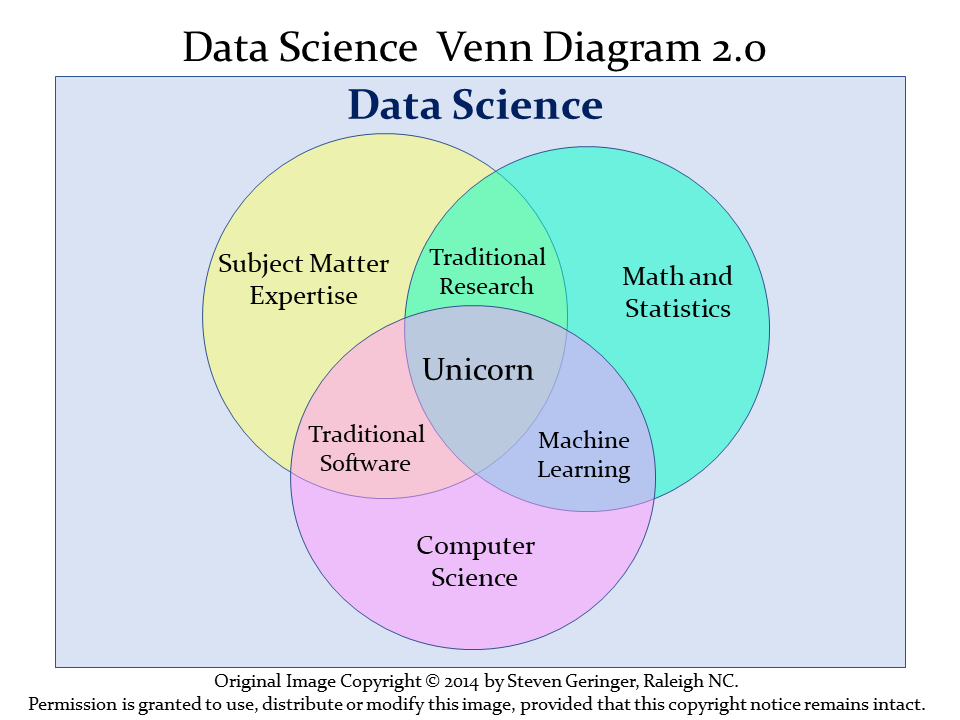
\includegraphics[width=0.8\linewidth]{figures/data-science-venn20} \caption{Data Science Venn Diagram from Steven Geringer}\label{fig:datasci-fig}
\end{figure}

\begin{itemize}
\tightlist
\item
  The field encompasses ideas from mathematics and statistics and from computer science, but with a heavy reliance on subject-matter knowledge. In our case, this includes clinical, health-related, medical or biological knowledge.
\item
  As \citet{Gelman-Nolan} suggest, the experience and intuition necessary for good statistical practice are hard to obtain, and teaching data science provides an excellent opportunity to reinforce statistical thinking skills across the full cycle of a data analysis project.
\item
  The principal form in which computer science (coding/programming) play a role in this course is to provide a form of communication. You'll need to learn how to express your ideas not just orally and in writing, but also through your code.
\end{itemize}

Data Science is a \textbf{team} activity. Everyone working in data science brings some part of the necessary skillset, but no one person can cover all three areas alone for excellent projects.

\begin{quote}
{[}The individual who is truly expert in all three key areas (mathematics/statistics, computer science and subject-matter knowledge) is{]} a mythical beast with magical powers who's rumored to exist but is never actually seen in the wild.

\url{http://www.kdnuggets.com/2016/10/battle-data-science-venn-diagrams.html}
\end{quote}

\hypertarget{data-science-project-cycle}{%
\section{Data Science Project Cycle}\label{data-science-project-cycle}}

A typical data science project can be modeled as follows, which comes from the introduction to the amazing book \textbf{R for Data Science}, by Garrett Grolemund and Hadley Wickham, which is a key text for this course \citep{R4DS}.

\begin{figure}
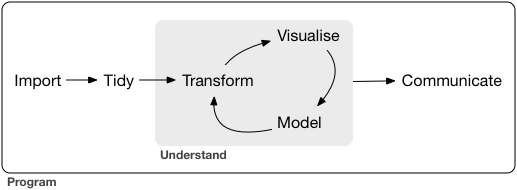
\includegraphics[width=0.95\linewidth]{figures/data-science-cycle} \caption{Source: R for Data Science: Introduction}\label{fig:cycle-fig}
\end{figure}

This diagram is sometimes referred to as the Krebs Cycle of Data Science. For more on the steps of a data science project, we encourage you to read the Introduction of \citet{R4DS}.

\hypertarget{data-science-and-the-431-course}{%
\section{Data Science and the 431 Course}\label{data-science-and-the-431-course}}

We'll discuss each of these elements in the 431 course, focusing at the start on understanding our data through transformation, modeling and (especially in the early stages) visualization. In 431, we learn how to get things done.

\begin{itemize}
\tightlist
\item
  We get people working with R and R Studio and R Markdown, even if they are completely new to coding. A gentle introduction is provided at \citet{ModernDive}
\item
  We learn how to use the \texttt{tidyverse} (\url{http://www.tidyverse.org/}), an array of tools in R (mostly developed by Hadley Wickham and his colleagues at R Studio) which share an underlying philosophy to make data science faster, easier, more reproducible and more fun. A critical text for understanding the tidyverse is \citet{R4DS}. Tidyverse tools facilitate:

  \begin{itemize}
  \tightlist
  \item
    \textbf{importing} data into R, which can be the source of intense pain for some things, but is really quite easy 95\% of the time with the right tool.
  \item
    \textbf{tidying} data, that is, storing it in a format that includes one row per observation and one column per variable. This is harder, and more important, than you might think.
  \item
    \textbf{transforming} data, perhaps by identifying specific subgroups of interest, creating new variables based on existing ones, or calculating summaries.
  \item
    \textbf{visualizing} data to generate actual knowledge and identify questions about the data - this is an area where R really shines, and we'll start with it in class.
  \item
    \textbf{modeling} data, taking the approach that modeling is complementary to visualization, and allows us to answer questions that visualization helps us identify.
  \item
    and last, but definitely not least, \textbf{communicating} results, models and visualizations to others, in a way that is reproducible and effective.
  \end{itemize}
\item
  Some programming/coding is an inevitable requirement to accomplish all of these aims. If you are leery of coding, you'll need to get past that, with the help of this course and our stellar teaching assistants. Getting started is always the most challenging part, but our experience is that most of the pain of developing these new skills evaporates by early October.
\end{itemize}

\hypertarget{what-the-course-is-and-isnt}{%
\section{What The Course Is and Isn't}\label{what-the-course-is-and-isnt}}

The 431 course is about \textbf{getting things done}. In developing this course, we adopt a modern approach that places data at the center of our work. Our goal is to teach you how to do truly reproducible research with modern tools. We want you to be able to collect and use data effectively to address questions of interest.

The curriculum includes more on several topics than you might expect from a standard graduate introduction to biostatistics.

\begin{itemize}
\tightlist
\item
  data gathering
\item
  data wrangling
\item
  exploratory data analysis and visualization
\item
  multivariate modeling
\item
  communication
\end{itemize}

It also nearly completely avoids formalism and is extremely applied - this is absolutely \textbf{not} a course in theoretical or mathematical statistics, and these Notes reflect that approach.

There's very little of the mathematical underpinnings here:

\[
f(x) = \frac{e^{-(x - \mu)^{2}/(2\sigma^{2})}}{\sigma{\sqrt{2 \pi }}} 
\]

Instead, these notes (and the course) focus on how we get R to do the things we want to do, and how we interpret the results of our work. Our next Chapter provides a first example.

  \bibliography{book.bib,packages.bib}

\end{document}
